% Chapter 5

\chapter{TR-069 Client} % Main chapter title

\label{Chapter5} % For referencing the chapter elsewhere, use \ref{Chapter5}

\lhead{Chapter 5. \emph{TR-069 Client}} % This is for the header on each page - perhaps a shortened title

TR-069 Client is implemented by Orange at 2008, but is a generic version for all potenial devices. The first part of my internship is to make TR-069 Client for Homelive Box. To be able to provide a generic TR-069 mudule which is easily portable on different devices, it satisfy the following points:

\begin{itemize}
  \item Written in ANSI C
  \item Small memory footprint
  \item Provide generic API to access device specific modules
  \item Provide Makefiles to build the binary
  \item Provide system traces on module activity
\end{itemize}
%----------------------------------------------------------------------------------------
\section{Architecture of TR-069 Client}
The TR069 Generic Agent is composed of several modules and interfaces. Some modules are generic and can be ported with no modification. Other modules are patform specific (specific libraries usage, specific device API to get/set values, ...) and must implement services declared into generic interfaces.

\begin{figure}[htbp]
	\centering
		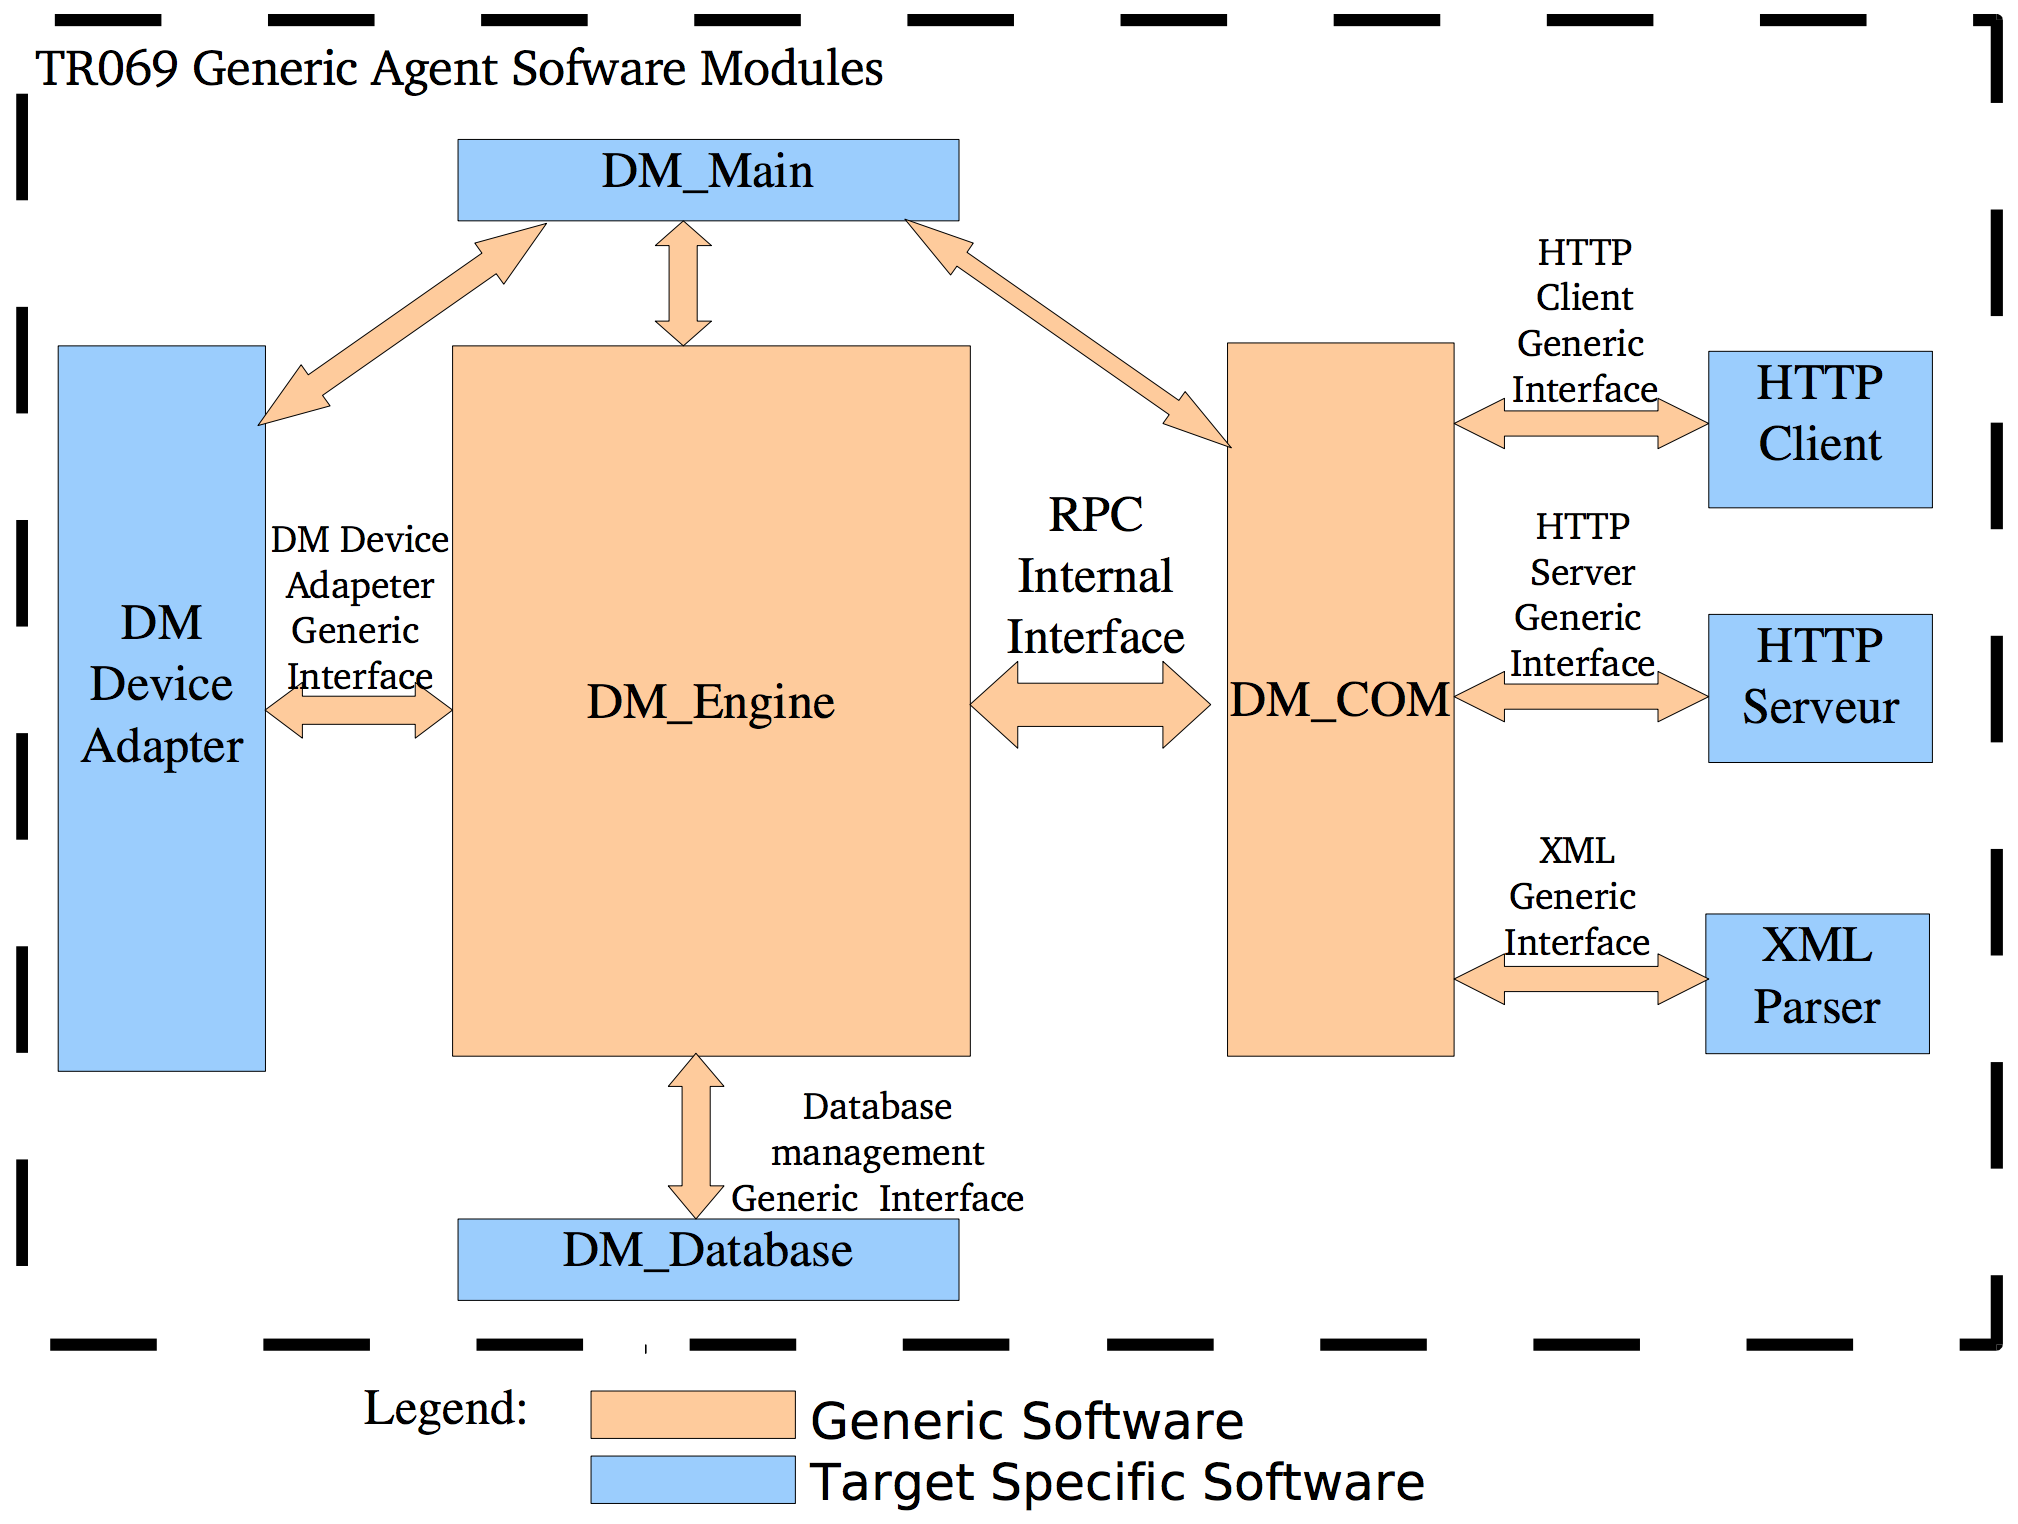
\includegraphics[width=12cm]{Figures/structuretr069.png}
	\caption[TR-069 Structure]{TR-069 Structure}
	\label{fig:tr069}
\end{figure}

For each module:
\begin{itemize}
  \item \textbf{DM_Engine} : In charge of the TR-069 logic,
  \item \textbf{DM_Com} : Handles the HTTP, SOAP and SSL Protocol with the ACS (Auto Configuration Server),
  \item \textbf{DM_DeviceAdapter} : Adaptation layer between the DM_Engine and the device system. It allows the implementation of the RPC commands (Get Parameter Value, Set Parameter Value, Reboot, Download, ...),
  \item \textbf{DM_Database} : Stores the data using an available storage solution on the device (or thanks to simple file storage),
  \item \textbf{HTTP Client} : Sets up / releases the HTTP connection with the ACS and sends / receives SOAP messages. The HTTP Client also handles SSL protocol,
  \item \textbf{HTTP SERVER} : Perform ACS Connection Request response,
  \item \textbf{XML Parser} : Decode / encode SOAP messages.
\end{itemize}

The figure below shows the file of the project, TR-069 Client defines all functions and APIs at each module. In consideration of easily ported to other devices, it put all target-related implementations in the folder \textit{dm_taget_implementation}.

\begin{figure}[htbp]
	\centering
		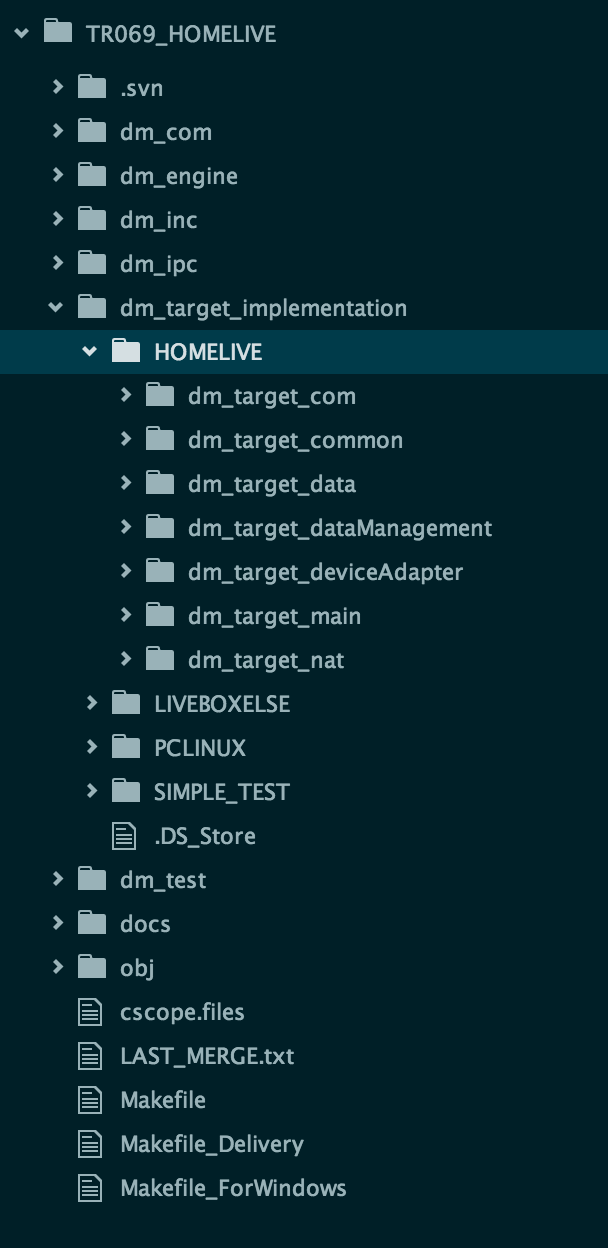
\includegraphics[width=8cm]{Figures/tr069_files.png}
	\caption[TR-069 File Tree Structure]{TR-069 File Tree Structure}
	\label{fig:tr069file}
\end{figure}


%----------------------------------------------------------------------------------------

\section{Problems and Solutions}

When 

%----------------------------------------------------------------------------------------
